\documentclass[xcolor=pdflatex,dvipsnames,table]{beamer}
\usepackage{epsfig,graphicx}
\usepackage{palatino}
\usepackage{fancybox}
\usepackage{relsize}
\usepackage[procnames]{listings}
\usepackage{hyperref}
\usepackage{qtree} % needed?
\usepackage{booktabs}
\usepackage{dirtree}
\usepackage[normalem]{ulem}


% fatter TT font
\renewcommand*\ttdefault{txtt}
% another TT, suggested by Alex
% \usepackage{inconsolata}
% \usepackage[T1]{fontenc} % needed as well?


\newcommand{\scale}{0.7}

\newcommand{\todo}[1]{{\emph{TODO: #1}}}
\newcommand{\martin}[1]{{\color{blue} Martin: #1}}
\newcommand{\abcdef}[1]{{\color{red} Author2: #1}}

% uncomment following for final submission
%\renewcommand{\todo}[1]{}
%\renewcommand{\martin}[1]{}
%\renewcommand{\author2}[1]{}

\newcommand{\code}[1]{{\texttt{#1}}}

\hypersetup{
  linkcolor  = black,
%  citecolor  = blue,
  urlcolor   = blue,
  colorlinks = true,
}

\beamertemplatenavigationsymbolsempty
\setbeamertemplate{footline}[frame number]





\newif\ifbook
% shared in slides and book

\lstdefinelanguage{chisel}{
  morekeywords={abstract,case,catch,class,def,%
    do,else,extends,false,final,finally,%
    for,if,implicit,import,match,mixin,%
    new,null,object,override,package,%
    private,protected,requires,return,sealed,%
    super,this,throw,trait,true,try,%
    type,val,var,while,with,yield},
  otherkeywords={=>,<-,<\%,<:,>:,\#,@},
  sensitive=true,
  morecomment=[l]{//},
  morecomment=[n]{/*}{*/},
  morestring=[b]",
  morestring=[b]',
  morestring=[b]"""
}

\usepackage{color}
\definecolor{dkgreen}{rgb}{0,0.6,0}
\definecolor{gray}{rgb}{0.5,0.5,0.5}
\definecolor{mauve}{rgb}{0.58,0,0.82}

% Default settings for code listings
\ifbook
\lstset{%frame=lines,
  language=chisel,
  aboveskip=3mm,
  belowskip=3mm,
  showstringspaces=false,
  columns=fixed, % basewidth=\mybasewidth,
  basicstyle={\small\ttfamily},
  numbers=none,
  numberstyle=\footnotesize,
  % identifierstyle=\color{red},
  breaklines=true,
  breakatwhitespace=true,
  procnamekeys={def, val, var, class, trait, object, extends},
  % procnamestyle=\ttfamily,
  tabsize=2,
  float
}
\else
\lstset{%frame=lines,
  language=chisel,
  aboveskip=3mm,
  belowskip=3mm,
  showstringspaces=false,
  columns=fixed, % basewidth=\mybasewidth,
  basicstyle={\small\ttfamily},
  numbers=none,
  numberstyle=\footnotesize\color{gray},
  % identifierstyle=\color{red},
  keywordstyle=\color{blue},
  commentstyle=\color{dkgreen},
  stringstyle=\color{mauve},
  breaklines=true,
  breakatwhitespace=true,
  procnamekeys={def, val, var, class, trait, object, extends},
  procnamestyle=\ttfamily\color{red},
  tabsize=2,
  float
}
\fi

\lstnewenvironment{chisel}[1][]
{\lstset{language=chisel,#1}}
{}

\newcommand{\shortlist}[1]{{\lstinputlisting[nolol]{#1}}}

\newcommand{\longlist}[3]{{\lstinputlisting[float, caption={#2}, label={#3}, frame=tb, captionpos=b]{#1}}}

\newcommand{\verylonglist}[3]{{\lstinputlisting[caption={#2}, label={#3}, frame=tb, captionpos=b]{#1}}}


\title{Testing and Verification}
\author{Martin Schoeberl}
\date{\today}
\institute{Technical University of Denmark\\
Embedded Systems Engineering}

\begin{document}

\begin{frame}
\titlepage
\end{frame}

\begin{frame}[fragile]{Overview}
\begin{itemize}
\item Synopsis and Syosil presentation on verification
\item Review components
\item Debugging and testing
\item Digital designers call testing verification
\begin{itemize}
\item To distinguish from final chip testing
\end{itemize}
\end{itemize}
\end{frame}

\begin{frame}[fragile]{Last Lab}
\begin{itemize}
\item On components and small sequential circuits
\begin{itemize}
\item Registers plus combinational circuits
\end{itemize}
\item Did you finish the exercises?
\item They are not mandatory, but helpful for preparation for the final project
\item Let's look at solutions
\end{itemize}
\end{frame}

\begin{frame}[fragile]{Components/Modules}
\begin{itemize}
\item Components are building blocks
\item Components have input and output ports (= pins)
\begin{itemize}
\item Organized as a \code{Bundle}
\item assigned to field \code{io}
\end{itemize}
\item We build circuits as a hierarchy of components
\begin{itemize}
\item You did a 4:1 multiplexer out of 3 2:1 mulitplexers
\end{itemize}
\item In Chisel a component is called \code{Module}
\item Components/Modules are used to organize the circuit
\begin{itemize}
\item Similar as using methods in Java
\end{itemize}
\end{itemize}
\end{frame}

\begin{frame}[fragile]{Hierarchy of Components Example}
\begin{figure}
  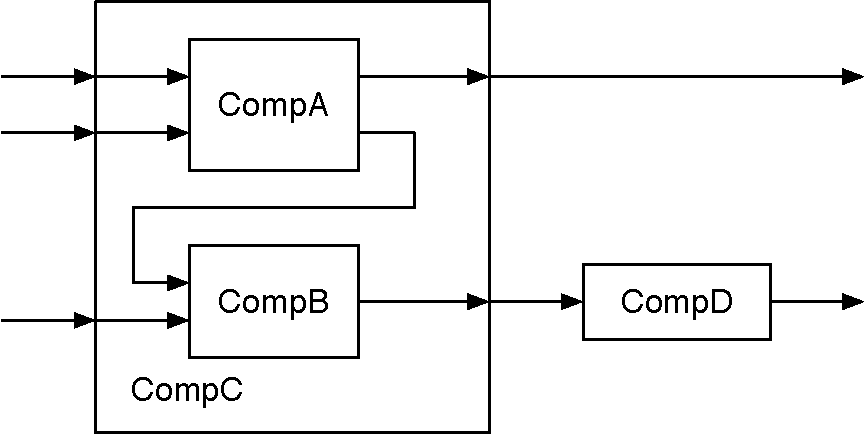
\includegraphics[scale=\scale]{../figures/components}
\end{figure}
\end{frame}


\begin{frame}[fragile]{Ports}
\begin{itemize}
\item Ports are the connections of modules
\item Ports are bundles with a direction
\item The direction be reversed with \code{Flipped}
\end{itemize}
\begin{chisel}
class Channel extends Bundle {
  val data = Input(UInt(32.W))
  val ready = Output(Bool())
  val valid = Input(Bool())
}

class ChannelUsage extends Bundle {
  val input = new Channel()
  val output = Flipped(new Channel())
}
\end{chisel}
\end{frame}

\begin{frame}[fragile]{An Adder Module}
\begin{itemize}
\item A \code{class} that \code{extends} \code{Module}
\item Interface (port) is a \code{Bundle}, wrapped into an \code{IO()}, and stored in the field \code{io}
\item Circuit description in the constructor
\end{itemize}
\begin{chisel}
class Adder extends Module {
  val io = IO(new Bundle {
    val a = Input(UInt(4.W))
    val b = Input(UInt(4.W))
    val result = Output(UInt(4.W))
  })

  val addVal = io.a + io.b
  io.result := addVal
}
\end{chisel}
\end{frame}


\begin{frame}[fragile]{Connections}
\begin{itemize}
\item Simple connections just with assignments, e.g.,
\begin{chisel}
  adder.io.a := ina
  adder.io.b := inb
\end{chisel}
\item Automatic bulk connections between components
\begin{chisel}
  dec.io <> exe.io
  mem.io <> exe.io
\end{chisel}
\end{itemize}
\end{frame}

\begin{frame}[fragile]{Module Usage}
\begin{itemize}
\item Create with \code{new} and wrap into a \code{Module()}
\item Interface port via the \code{io} field
\item Note the assignment operator \code{:=} on \code{io} fields
\end{itemize}
\begin{chisel}
  val adder = Module(new Adder())
  adder.io.a := ina
  adder.io.b := inb
  val result = adder.io.result
\end{chisel}
\end{frame}


\begin{frame}[fragile]{Chisel Main}

\begin{itemize}
\item Create one top-level Module
\item Invoke the Chisel driver from the App
\item Pass the top module (e.g., \code{new Hello()})
\item Optional: pass some parameters (in the \code{Array})
\item Following code generates Verilog code for \emph{Hello World}
\end{itemize}
\begin{chisel}
object Hello extends App {
  chisel3.Driver.execute(Array[String](), () => new Hello())
}
\end{chisel}
\end{frame}




\begin{frame}[fragile]{Midterm Evaluation}
\begin{itemize}
\item An anonymous Google form (no login required)
\item 20 minutes time, including the break
\item We will look into it after the break
\end{itemize}
\begin{figure}
  
\includegraphics[scale=0.5]{forms2020}
\end{figure}
\begin{itemize}
\item \url{https://forms.gle/wtvDrA4peD4oLvt16}
\end{itemize}
\end{frame}

\begin{frame}[fragile]{Testing and Debugging}
\begin{itemize}
\item Nobody writes perfect code ;-)
\item We need a method to improve the code
\item In Java we can simply print the result:
\begin{itemize}
\item \code{println("42");}
\end{itemize}
\item What can we do in hardware?
\begin{itemize}
\item Describe the whole circuit and hope it works?
\item We can switch an LED on or off
\end{itemize}
\item We need some tools for \href{https://en.wikipedia.org/wiki/Debugging#/media/File:H96566k.jpg}{debugging}
\item Writing testers in Chisel
\end{itemize}
\end{frame}

\begin{frame}[fragile]{Testing with Chisel}
\begin{itemize}
\item Set input values with \code{poke}
\item Advance the simulation with \code{step}
\item Read the output values with \code{peek}
\item Compare the values with \code{expect}
\item Import following packages:
\shortlist{../code/test_import.txt}
\end{itemize}
\end{frame}

\begin{frame}[fragile]{Using \code{peek}, \code{poke}, and \code{expect}}
\begin{chisel}
// Set input values
poke(dut.io.a, 3)
poke(dut.io.b, 4)
// Execute one iteration
step(1)
// Print the result
val res = peek(dut.io.result)
println(res)

// Or compare against expected value
expect(dut.io.result, 7)
\end{chisel}
\end{frame}

\begin{frame}[fragile]{A Chisel Tester}
\begin{itemize}
\item Extends class \code{PeekPokeTester}
\item Has the device-under test (DUT) as parameter
\item Testing code can use all features of Scala
\end{itemize}
\begin{chisel}
class CounterTester(dut: Counter) extends PeekPokeTester(dut) {

  // Here comes the Chisel/Scala code
  // for the testing
}
\end{chisel}
\end{frame}

\begin{frame}[fragile]{Example DUT}
\begin{itemize}
\item A device-under test (DUT)
\shortlist{../code/test_dut.txt}
\end{itemize}
\end{frame}

\begin{frame}[fragile]{A Simple Tester}
\begin{itemize}
\item Just using \code{println} for manual inspection
\shortlist{../code/test_bench_simple.txt}
\end{itemize}
\end{frame}


\begin{frame}[fragile]{The Main Program for the Test}
\begin{itemize}
\item Extend an App and invoke the \code{iotesters} driver
\item With the DUT and the tester
\shortlist{../code/test_main_simple.txt}
\end{itemize}
\end{frame}

\begin{frame}[fragile]{A Real Tester}
\begin{itemize}
\item Poke values and \code{expect} some output
\shortlist{../code/test_bench.txt}
\end{itemize}
\end{frame}

\begin{frame}[fragile]{ScalaTest}
\begin{itemize}
\item Testing framework for Scala
\item \code{sbt} understands ScalaTest
\item Run all tests:
\code{sbt test}
\item When all \code{expect}s are ok, the test passes
\item A little bit funny syntax
\item Add library to \code{build.sbt}
\begin{chisel}
libraryDependencies += "org.scalatest" %% "scalatest" % "3.0.5" % "test"
\end{chisel}
\item Import ScalaTest library
\begin{chisel}
import org.scalatest._
\end{chisel}
\end{itemize}
\end{frame}

\begin{frame}[fragile]{ScalaTest Version of our Tester}
\shortlist{../code/scalatest_simple.txt}
\end{frame}

\begin{frame}[fragile]{Generating Waveforms}
\begin{itemize}
\item Waveforms are timing diagrams
\item Good to see many parallel signals and registers
\item Additional parameters: \code{"--generate-vcd-output", "on"}
\item IO signals and registers are dumped
\item Option \code{--debug} puts all wires into the dump
\item Generates a .vcd file
\item Viewing with GTKWave or ModelSim
\end{itemize}
\end{frame}


\begin{frame}[fragile]{Waveform Testing Demo}
\begin{itemize}
\item Counter with a limit from last week (\code{Count6})
\item Show Count6 tester: the original and the waveform
\item Run it and look at waveform
\item Add the solution
\item Run again and reload the waveform
\end{itemize}
\end{frame}

\begin{frame}[fragile]{A Self-Running Circuit}
\begin{itemize}
\item \code{Count6} is a self-running circuit
\item Needs no stimuli (\code{poke})
\item Just run for a few cycles
\end{itemize}
\begin{chisel}
class Count6Wave(dut: Count6) extends PeekPokeTester(dut) {
  step(20)
}
\end{chisel}
\end{frame}

\begin{frame}[fragile]{Call the Tester}
\begin{itemize}
\item Using here ScalaTest
\item Note \code{Driver.execute}
\item Note \code{Array("--generate-vcd-output", "on")}
\end{itemize}
\begin{chisel}
class Count6WaveSpec extends
  FlatSpec with Matchers {
  
  "CountWave6 " should "pass" in {
    chisel3.iotesters.Driver.
    execute(Array("--generate-vcd-output", "on"),() => new Count6)
    { c => new Count6Wave(c) }
    should be (true)
  }
}
\end{chisel}
\end{frame}

\begin{frame}[fragile]{Vending Machine Testing}
\begin{itemize}
\item I provide a minimal tester to generate a waveform
\item Adding some coins and buying
\item You can and shall extend this tester
\item Better having more than one tester
\item Show the waveform of the working VM
\end{itemize}
\end{frame}



\begin{frame}[fragile]{Test Driven Development (TDD)}
\begin{itemize}
\item Software development process
\begin{itemize}
\item Can we learn from SW development for HW design?
\end{itemize}
\item Writing the test first, then the implementation
\item Started with extreme programming
\begin{itemize}
\item Frequent releases
\item Accept change as part of the development
\end{itemize}
\item Not used in its pour form
\begin{itemize}
\item Writing all those tests is simply considerer too much work
\end{itemize}
\end{itemize}
\end{frame}

\begin{frame}[fragile]{Regresssion Tests}
\begin{itemize}
\item But tests are collected over time
\item When a bug is found, a test is written to reproduce this bug
\item Collection of tests increases
\item Runs every night to test for \emph{regression}
\begin{itemize}
\item Did a code change introduce a bug in the current code base?
\end{itemize}
\end{itemize}
\end{frame}


\begin{frame}[fragile]{Continuous Integration (CI)}
\begin{itemize}
\item Next logical step from regression tests
\item Run all tests whenever code is changed
\item Automate this with a repository, e.g., on GitHub
\item Run CI on Travis (with GitHub integration)
\item Show about this on the Chisel book
\begin{itemize}
\item Show \code{sbt test}
\item Mails from travis
\item Live demo on travis
\end{itemize}
\item \url{https://travis-ci.com/schoeberl/chisel-book}
\end{itemize}
\end{frame}


\begin{frame}[fragile]{Testing versus Debugging}
\begin{itemize}
\item Debugging is during code development
\item Waveform and println are easy tools for debugging
\item Debugging does not help for regression tests
\item Write small test cases for regression tests
\item Keeps your code base \emph{intact} when doing changes
\item Better confidence in changes not introducing new bugs
\end{itemize}
\end{frame}

\begin{frame}[fragile]{Scala Build Tool (sbt)}
\begin{itemize}
\item Downloads Scala compiler if needed
\item Downloads dependent libraries (e.g., Chisel)
\item Compiles Scala programs
\item Executes Scala programs
\item Does a lot of magic, maybe too much
\item Compile and run with:
\end{itemize}
\begin{chisel}
sbt "runMain simple.Example"
sbt run
sbt test
sbt "testOnly MySpec"
sbt compile
\end{chisel}
\end{frame}

\begin{frame}[fragile]{Build Configuration}
\begin{itemize}
\item Defines needed Scala version
\item Library dependencies
\item File name: \code{build.sbt}
\end{itemize}
\begin{chisel}
scalaVersion := "2.11.7"

resolvers ++= Seq(
  Resolver.sonatypeRepo("snapshots"),
  Resolver.sonatypeRepo("releases")
)

libraryDependencies += "edu.berkeley.cs" %% "chisel3" % "3.1.2"
libraryDependencies += "edu.berkeley.cs" %% "chisel-iotesters" % "1.2.2"
\end{chisel}
\end{frame}

\begin{frame}[fragile]{Today's Lab}
\begin{itemize}
\item Binary to 7-segment decoder
\item First part of your vending machine
\item Just a single digit, only combinational logic
\item Use the nice tester provided to develop the circuit
\item Then synthesize it for the FPGA
\item Test with switches
\item Show a TA your working design
\item \href{https://github.com/schoeberl/chisel-lab/tree/master/lab5}{Lab 5}
\end{itemize}
\end{frame}

\begin{frame}[fragile]{Summary}
\begin{itemize}
\item Small sequential circuits are our building blocks
\item We build larger circuits by combining components (moduls)
\item There is no \emph{println} in hardware
\item We need to write tests for the development
\item Debugging versus regression tests
\end{itemize}
\end{frame}


\end{document}

